% Practice Test 09 — Texas Edition
% Questions: 30 (21 MC + 9 SA)
% Generated by scripts/generate_practice_tests.py

\begin{practiceQuestion}{1-3-q14}{mc}
\begin{questionText}
A recipe uses cups of flour proportional to servings. If $12$ servings need $9$ cups, what is $k$ in cups per serving?
\end{questionText}
\choiceA{$\frac{3}{4}$}
\choiceB{$\frac{4}{3}$}
\choiceC{$3$}
\choiceD{$9$}
\correctAnswer{A}
\explanation{$k = \frac{9}{12} = \frac{3}{4}$ cups per serving.}
\end{practiceQuestion}

\begin{practiceQuestion}{1-6-q10}{mc}
\begin{questionText}
A recipe uses $2\frac{1}{2}$ cups of flour to make $30$ cookies. How many cups are needed for $48$ cookies?
\end{questionText}
\choiceA{$3$ cups}
\choiceB{$3\frac{1}{2}$ cups}
\choiceC{$4$ cups}
\choiceD{$4\frac{1}{2}$ cups}
\correctAnswer{C}
\explanation{$\frac{2.5}{30} = \frac{x}{48}$. Cross-multiply: $30x = 120$, so $x = 4$ cups.}
\end{practiceQuestion}

\begin{practiceQuestion}{2-1-q23}{sa}
\begin{questionText}
A farmer planted $180$ trees and $126$ survived. What percent of the trees survived?
\end{questionText}
\correctAnswer{$70\%$}
\explanation{Divide: $126 \div 180 = 0.70 = 70\%$.}
\end{practiceQuestion}

\begin{practiceQuestion}{2-3-q02}{mc}
\begin{questionText}
A population grew from $5{,}000$ to $5{,}750$. What is the percent increase?
\end{questionText}
\choiceA{$12\%$}
\choiceB{$13\%$}
\choiceC{$15\%$}
\choiceD{$17.5\%$}
\correctAnswer{C}
\explanation{Change: $5{,}750 - 5{,}000 = 750$. Percent change: $750 \div 5{,}000 = 0.15 = 15\%$.}
\end{practiceQuestion}

\begin{practiceQuestion}{2-6-q15}{mc}
\begin{questionText}
After $3$ years at $4\%$ simple interest, an account has $\$672$. What was the original deposit?
\end{questionText}
\choiceA{$\$500$}
\choiceB{$\$560$}
\choiceC{$\$600$}
\choiceD{$\$650$}
\correctAnswer{C}
\explanation{Total $= P + Prt = P(1 + rt) = P(1 + 0.04 \times 3) = 1.12P$. So $672 = 1.12P$ → $P = \$600$.}
\end{practiceQuestion}

\begin{practiceQuestion}{2-8-q06}{mc}
\begin{questionText}
Which statement about a debit card is TRUE?
\end{questionText}
\choiceA{You borrow money and pay it back later}
\choiceB{You must pay interest on every purchase}
\choiceC{You spend money that is already in your account}
\choiceD{You can spend more than your account balance}
\correctAnswer{C}
\explanation{A debit card draws directly from funds you already have in your checking account.}
\end{practiceQuestion}

\begin{practiceQuestion}{2-9-q21}{sa}
\begin{questionText}
Your clothing budget is $\$200$ per month. You spend $\$230$. By what percent did you go over budget?
\end{questionText}
\correctAnswer{$15\%$}
\explanation{Over by $\$30$. Percent: $\frac{30}{200} = 0.15 = 15\%$.}
\end{practiceQuestion}

\begin{practiceQuestion}{2-10-q07}{mc}
\begin{questionText}
You deposit $\$200$ at $8\%$ compounded yearly. What is the amount after $1$ year?
\end{questionText}
\choiceA{$\$208$}
\choiceB{$\$216$}
\choiceC{$\$280$}
\choiceD{$\$216.32$}
\correctAnswer{B}
\explanation{$200 \times 1.08 = \$216$.}
\end{practiceQuestion}

\begin{practiceQuestion}{4-1-q19}{sa}
\begin{questionText}
Write an expression for ``$9$ less than the quotient of a number $m$ and $5$.''
\end{questionText}
\correctAnswer{$\frac{m}{5} - 9$}
\explanation{``The quotient of $m$ and $5$'' is $\frac{m}{5}$. ``$9$ less than'' means subtract $9$: $\frac{m}{5} - 9$.}
\end{practiceQuestion}

\begin{practiceQuestion}{4-2-q28}{gmc}
\begin{questionText}
Look at the two groups of algebra tiles below. Which expression represents their sum?

\begin{center}
\begin{tikzpicture}[scale=0.55]
  % Group 1 label
  \node[font=\bfseries] at (3, 1.5) {Group 1};
  \fill[funBlue!40] (0,0) rectangle (2,1);
  \draw[thick] (0,0) rectangle (2,1);
  \node at (1,0.5) {$x$};
  \fill[funBlue!40] (2.3,0) rectangle (4.3,1);
  \draw[thick] (2.3,0) rectangle (4.3,1);
  \node at (3.3,0.5) {$x$};
  \fill[funGreen!40] (4.8,0) rectangle (5.8,1);
  \draw[thick] (4.8,0) rectangle (5.8,1);
  \node at (5.3,0.5) {$1$};

  % Group 2 label
  \node[font=\bfseries] at (3, -1) {Group 2};
  \fill[funBlue!40] (0,-2.5) rectangle (2,-1.5);
  \draw[thick] (0,-2.5) rectangle (2,-1.5);
  \node at (1,-2) {$x$};
  \fill[funGreen!40] (2.5,-2.5) rectangle (3.5,-1.5);
  \draw[thick] (2.5,-2.5) rectangle (3.5,-1.5);
  \node at (3,-2) {$1$};
  \fill[funGreen!40] (3.8,-2.5) rectangle (4.8,-1.5);
  \draw[thick] (3.8,-2.5) rectangle (4.8,-1.5);
  \node at (4.3,-2) {$1$};
  \fill[funGreen!40] (5.1,-2.5) rectangle (6.1,-1.5);
  \draw[thick] (5.1,-2.5) rectangle (6.1,-1.5);
  \node at (5.6,-2) {$1$};
\end{tikzpicture}
\end{center}
\end{questionText}
\choiceA{$3x + 3$}
\choiceB{$2x + 4$}
\choiceC{$3x + 4$}
\choiceD{$2x + 3$}
\correctAnswer{C}
\explanation{Group 1: $2x + 1$. Group 2: $x + 3$. Sum: $(2x + 1) + (x + 3) = 3x + 4$.}
\end{practiceQuestion}

\begin{practiceQuestion}{5-3-q26}{gmc}
\begin{questionText}
The rectangle below has an area of $56$ square cm. What is the value of $x$?

\begin{center}
\begin{tikzpicture}[scale=0.7]
  \draw[thick,fill=funBlue!10] (0,0) rectangle (7,3);
  \draw[<->] (0,-0.5) -- (7,-0.5);
  \node[below] at (3.5,-0.5) {$7$ cm};
  \draw[<->] (-0.5,0) -- (-0.5,3);
  \node[left] at (-0.5,1.5) {$(x + 3)$ cm};
\end{tikzpicture}
\end{center}
\end{questionText}
\choiceA{$x = 5$}
\choiceB{$x = 8$}
\choiceC{$x = 11$}
\choiceD{$x = 4$}
\correctAnswer{A}
\explanation{Area $= 7(x + 3) = 56$. Divide by $7$: $x + 3 = 8$. Subtract $3$: $x = 5$.}
\end{practiceQuestion}

\begin{practiceQuestion}{5-4-q03}{mc}
\begin{questionText}
Solve $0.25n - 1.5 = 3.5$.
\end{questionText}
\choiceA{$n = 8$}
\choiceB{$n = 20$}
\choiceC{$n = 14$}
\choiceD{$n = 2$}
\correctAnswer{B}
\explanation{Add $1.5$: $0.25n = 5$. Divide by $0.25$: $n = 20$. Check: $0.25(20) - 1.5 = 5 - 1.5 = 3.5$ \checkmark.}
\end{practiceQuestion}

\begin{practiceQuestion}{5-5-q10}{mc}
\begin{questionText}
Solve $3x + 7 \leq 25$.
\end{questionText}
\choiceA{$x \leq \dfrac{32}{3}$}
\choiceB{$x \leq 6$}
\choiceC{$x \geq 6$}
\choiceD{$x \leq 9$}
\correctAnswer{B}
\explanation{Subtract $7$: $3x \leq 18$. Divide by $3$: $x \leq 6$.}
\end{practiceQuestion}

\begin{practiceQuestion}{5-6-q28}{gmc}
\begin{questionText}
Look at the two number lines below. Which statement is true?

\textbf{Line 1:}
\begin{center}
\begin{tikzpicture}[scale=0.55]
  \draw[thick,->] (-6,0) -- (6,0);
  \foreach \x in {-5,...,5} \draw (\x,0.12) -- (\x,-0.12) node[below,font=\small] {$\x$};
  \draw[thick,funBlue,->] (-3,0) -- (6,0);
  \fill[funBlue] (-3,0) circle (4pt);
\end{tikzpicture}
\end{center}

\textbf{Line 2:}
\begin{center}
\begin{tikzpicture}[scale=0.55]
  \draw[thick,->] (-6,0) -- (6,0);
  \foreach \x in {-5,...,5} \draw (\x,0.12) -- (\x,-0.12) node[below,font=\small] {$\x$};
  \draw[thick,funOrange,->] (-3,0) -- (6,0);
  \draw[thick,funOrange,fill=white] (-3,0) circle (4pt);
\end{tikzpicture}
\end{center}
\end{questionText}
\choiceA{Both graphs include $-3$ as a solution}
\choiceB{Line 1 shows $x \geq -3$ and Line 2 shows $x > -3$}
\choiceC{Line 1 shows $x > -3$ and Line 2 shows $x \geq -3$}
\choiceD{Both graphs represent the same inequality}
\correctAnswer{B}
\explanation{Line 1 has a closed circle (includes $-3$): $x \geq -3$. Line 2 has an open circle (excludes $-3$): $x > -3$.}
\end{practiceQuestion}

\begin{practiceQuestion}{6-2-q03}{mc}
\begin{questionText}
A model uses scale $1:100$. You need to redraw it at scale $1:50$. A wall that is $4$ cm on the original model becomes how long?
\end{questionText}
\choiceA{$2$ cm}
\choiceB{$4$ cm}
\choiceC{$8$ cm}
\choiceD{$200$ cm}
\correctAnswer{C}
\explanation{Scale ratio: $\frac{100}{50} = 2$. New length: $4 \times 2 = 8$ cm.}
\end{practiceQuestion}

\begin{practiceQuestion}{6-3-q05}{mc}
\begin{questionText}
Can a triangle have sides $6$, $8$, and $14$?
\end{questionText}
\choiceA{Yes, it is a right triangle}
\choiceB{Yes, it is an obtuse triangle}
\choiceC{No, the triangle inequality is not satisfied}
\choiceD{No, because the sides are all even numbers}
\correctAnswer{C}
\explanation{$6 + 8 = 14$, which is not greater than $14$. The sum must be strictly greater, so no triangle can be formed.}
\end{practiceQuestion}

\begin{practiceQuestion}{6-4-q02}{mc}
\begin{questionText}
A triangle has angles $40°$, $60°$, and $80°$. How many different triangles can be drawn?
\end{questionText}
\choiceA{None}
\choiceB{Exactly one}
\choiceC{Exactly three}
\choiceD{Infinitely many}
\correctAnswer{D}
\explanation{AAA determines the shape but not the size. Infinitely many similar triangles of different sizes share these angle measures.}
\end{practiceQuestion}

\begin{practiceQuestion}{6-5-q22}{sa}
\begin{questionText}
Name two different cross-section shapes you can get from slicing a cube.
\end{questionText}
\correctAnswer{Any two of: square, rectangle, triangle, pentagon, hexagon}
\explanation{A cube can be sliced to produce squares, rectangles, triangles, pentagons, or hexagons depending on the angle and position of the cut.}
\end{practiceQuestion}

\begin{practiceQuestion}{6-8-q29}{gsa}
\begin{questionText}
The two triangles below are similar. Find the missing side lengths $a$ and $b$.

\begin{center}
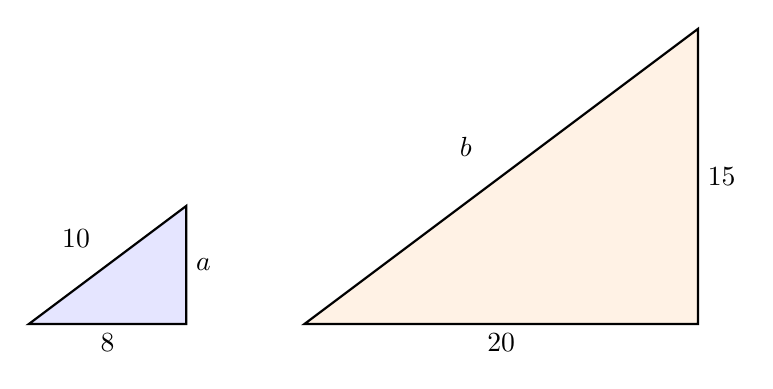
\begin{tikzpicture}[scale=0.5]
  % Small triangle
  \draw[thick,fill=blue!10] (0,0) -- (4,0) -- (4,3) -- cycle;
  \node[below] at (2,0) {$8$};
  \node[right] at (4,1.5) {$a$};
  \node[above left] at (1.8,1.7) {$10$};
  % Large triangle
  \draw[thick,fill=orange!10] (7,0) -- (17,0) -- (17,7.5) -- cycle;
  \node[below] at (12,0) {$20$};
  \node[right] at (17,3.75) {$15$};
  \node[above left] at (11.5,4) {$b$};
\end{tikzpicture}
\end{center}
\end{questionText}
\correctAnswer{$a = 6$, $b = 25$}
\explanation{Scale factor from small to large: $\frac{20}{8} = 2.5$. $a$: from large to small on the right side $= 15 \div 2.5 = 6$. $b$: from small to large on the hypotenuse $= 10 \times 2.5 = 25$.}
\end{practiceQuestion}

\begin{practiceQuestion}{7-4-q12}{mc}
\begin{questionText}
A square has sides of $10$ m. A quarter circle with radius $10$ m is removed from one corner. What is the area of the remaining figure? Use $\pi \approx 3.14$.
\end{questionText}
\choiceA{$21.5$ m$^2$}
\choiceB{$50$ m$^2$}
\choiceC{$78.5$ m$^2$}
\choiceD{$100$ m$^2$}
\correctAnswer{A}
\explanation{Square: $100$ m$^2$. Quarter circle: $\frac{1}{4} \times 3.14 \times 100 = 78.5$ m$^2$. Remaining: $100 - 78.5 = 21.5$ m$^2$.}
\end{practiceQuestion}

\begin{practiceQuestion}{7-5-q03}{mc}
\begin{questionText}
A rectangular box is $10$ in by $6$ in by $4$ in. What is the total surface area?
\end{questionText}
\choiceA{$120$ in$^2$}
\choiceB{$240$ in$^2$}
\choiceC{$248$ in$^2$}
\choiceD{$148$ in$^2$}
\correctAnswer{C}
\explanation{$SA = 2(10 \times 6) + 2(10 \times 4) + 2(6 \times 4) = 120 + 80 + 48 = 248$ in$^2$.}
\end{practiceQuestion}

\begin{practiceQuestion}{7-6-q23}{sa}
\begin{questionText}
A rectangular prism has a volume of $360$ cm$^3$. Its length is $12$ cm and its height is $5$ cm. What is its width?
\end{questionText}
\correctAnswer{$6$ cm}
\explanation{$360 = 12 \times w \times 5 = 60w$. $w = 360 \div 60 = 6$ cm.}
\end{practiceQuestion}

\begin{practiceQuestion}{8-1-q24}{sa}
\begin{questionText}
A random sample of $100$ out of $4{,}000$ residents found that $45$ support a new library. Predict how many residents support it.
\end{questionText}
\correctAnswer{$1{,}800$}
\explanation{$\frac{45}{100} = 45\%$. Then $45\%$ of $4{,}000 = 1{,}800$.}
\end{practiceQuestion}

\begin{practiceQuestion}{8-2-q19}{sa}
\begin{questionText}
A random sample of $50$ students found a mean score of $76$. Another sample of $50$ found a mean of $80$. Estimate the population mean.
\end{questionText}
\correctAnswer{$78$}
\explanation{Average the two sample means: $\frac{76+80}{2} = 78$.}
\end{practiceQuestion}

\begin{practiceQuestion}{8-4-q04}{mc}
\begin{questionText}
Which measure of variability focuses on the middle $50\%$ of the data?
\end{questionText}
\choiceA{Range}
\choiceB{Mean}
\choiceC{Interquartile range (IQR)}
\choiceD{Median}
\correctAnswer{C}
\explanation{IQR $= Q_3 - Q_1$ measures the spread of the middle $50\%$ of the data.}
\end{practiceQuestion}

\begin{practiceQuestion}{8-5-q01}{mc}
\begin{questionText}
In a stem-and-leaf plot, $5 \mid 3$ means:
\end{questionText}
\choiceA{$5.3$}
\choiceB{$35$}
\choiceC{$53$}
\choiceD{$5 + 3 = 8$}
\correctAnswer{C}
\explanation{The stem is the tens digit and the leaf is the ones digit, so $5 \mid 3$ means $53$.}
\end{practiceQuestion}

\begin{practiceQuestion}{8-6-q07}{mc}
\begin{questionText}
A circle graph shows these results for a survey of $200$ people: Red $30\%$, Blue $45\%$, Green $25\%$. How many chose blue?
\end{questionText}
\choiceA{$45$}
\choiceB{$60$}
\choiceC{$90$}
\choiceD{$100$}
\correctAnswer{C}
\explanation{$45\%$ of $200 = 0.45 \times 200 = 90$.}
\end{practiceQuestion}

\begin{practiceQuestion}{9-4-q25}{sa}
\begin{questionText}
A probability model assigns $P(A) = 0.35$, $P(B) = 0.25$, $P(C) = 0.25$, and $P(D) = 0.20$. Is this a valid model? Explain.
\end{questionText}
\correctAnswer{No}
\explanation{$0.35 + 0.25 + 0.25 + 0.20 = 1.05$, which is greater than $1$. A valid model must have probabilities that sum to exactly $1$.}
\end{practiceQuestion}

\begin{practiceQuestion}{9-6-q14}{mc}
\begin{questionText}
A bag has $4$ green and $6$ yellow marbles. You pick one marble without replacement and then pick another. What is the probability that the first is green and the second is yellow?
\end{questionText}
\choiceA{$\frac{24}{100}$}
\choiceB{$\frac{24}{90}$}
\choiceC{$\frac{4}{15}$}
\choiceD{$\frac{6}{10}$}
\correctAnswer{C}
\explanation{$P(\text{green first}) = \frac{4}{10}$. After removing a green, $P(\text{yellow second}) = \frac{6}{9}$. $P = \frac{4}{10} \times \frac{6}{9} = \frac{24}{90} = \frac{4}{15}$.}
\end{practiceQuestion}

\begin{practiceQuestion}{9-7-q06}{mc}
\begin{questionText}
Why are simulations useful?
\end{questionText}
\choiceA{They always give exact answers}
\choiceB{They can estimate probabilities when real experiments are too difficult or impractical}
\choiceC{They replace all mathematical calculations}
\choiceD{They only work for coin flips}
\correctAnswer{B}
\explanation{Simulations estimate probabilities for complex events that are hard to compute directly or where real experiments are impractical.}
\end{practiceQuestion}
